\chapter{Methods and Research Design}

This chapter describes the development, training, and evaluation of a Multi-Agent Reinforcement Learning (MARL) model for dynamic bus scheduling under non-ideal conditions. The goal is a reproducible pipeline from the public-data-calibrated CapMetro Route 801 direction-code 6 case to measurable controller performance under baseline and disturbed operating conditions.


\section{Research Design}

The study uses a \textbf{controlled comparative experimental design} with control strategy (No Control, Forward Headway, Even Headway, MARL) and the activation-matrix condition as factors. Conditions include the D+T Stage A baseline, the D+T+S+W+B combined evaluation, the S/W/B single-disturbance ablations, and the separate synthetic $\eta$ sweep. The response variables are simulated mean passenger waiting time, mean bus travel time, and headway coefficient of variation.

Each combination is replicated $N_{\mathrm{runs}} \geq 30$ times using independent Monte Carlo seeds. The unit of analysis is one full simulated operating day on Route 801 direction code 6. Random seeds and disturbance realizations are matched across control strategies within each evaluation cell, so paired performance differences reflect the controller rather than different stochastic draws \cite{Henderson2018Matters,Agarwal2021Precipice}. Bootstrap intervals are retained for heavy-tailed responses instead of treating the sample-size threshold alone as proof of normality.

Throughout, disturbances play two distinct roles that must not be conflated. During \textbf{training}, the full range of stochastic disturbances is always active, the policy is trained under domain randomization \cite{Tang2024Curriculum} so that it learns to act under demand surges, traffic friction, heavy-tailed weather delays, and breakdowns. During \textbf{evaluation}, the same generators are used to define two test conditions (ideal and non-ideal) that probe the \textit{already-trained} policy on disturbance realizations it did not see during training but which are drawn from the same generative process. The ideal/non-ideal split is therefore an \textbf{evaluation factor, not a training switch}: the agent is never trained on a disturbance-free corridor. 
\pagebreak
\section{Methodology}

\subsection{Simulation Environment}

The study uses a two-stage simulation architecture. \textbf{SUMO} (Simulation of Urban Mobility)~\cite{Lopez2018SUMO} serves as the \textbf{calibration layer}, providing a microscopic representation of Route 801 from which empirical parameters are extracted. A \textbf{custom Python environment built on the PettingZoo Agent Environment Cycle (AEC) API}~\cite{Terry2021PettingZoo} serves as the \textbf{training and Monte Carlo evaluation layer}, where MARL agents interact with a lightweight bus dynamics model parameterized by the calibrated distributions. SUMO is used for corridor calibration rather than for the full learning budget; all training and evaluation runs execute in the lighter event-driven environment.

PettingZoo's AEC API is chosen over three alternatives. First, the single-agent Gymnasium interface~\cite{Towers2024Gymnasium} cannot natively represent multiple agents acting on independent events. Fitting multi-agent control into a single-agent API requires either treating the entire fleet as one composite agent, which breaks parameter sharing, or coordinating agents manually outside the API, which removes the benefit of using a standard interface. Second, PettingZoo's parallel API assumes all agents step simultaneously~\cite{Terry2021PettingZoo}, which does not match asynchronous bus control where only the bus arriving at a control stop has a decision to make. Third, a fully custom implementation was considered but rejected because it would sacrifice compatibility with established algorithm libraries and complicate reproducibility. AEC handles the asynchronous case by cycling through one agent at a time rather than stepping all agents in parallel~\cite{Terry2021PettingZoo}. This matches the approach used by Wang and Sun~\cite{Wangsun} and Rodriguez et al.~\cite{Rodriguez2023Cooperative}, both of whom implemented the same asynchronous logic in custom event-driven simulators. Adopting AEC preserves their event-driven dynamics while providing a standardized interface compatible with parameter-sharing algorithm libraries.

\begin{figure}[htbp]
    \centering
    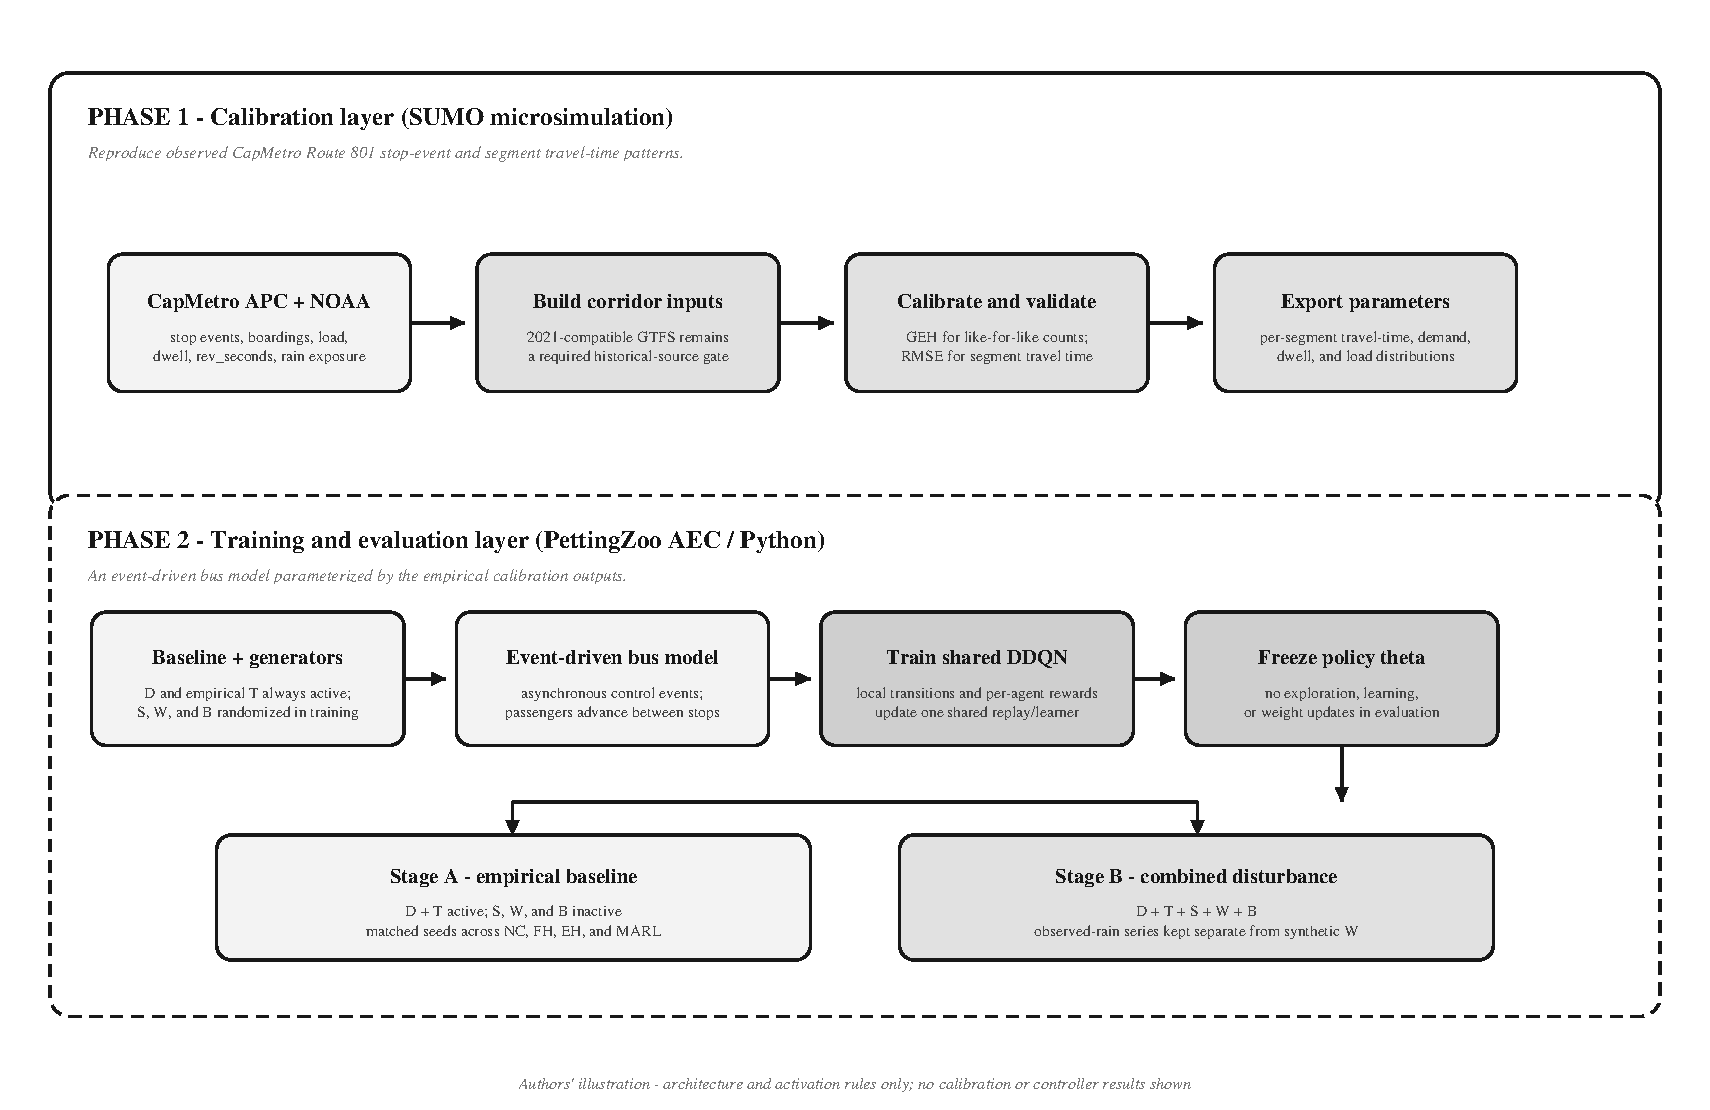
\includegraphics[width=\textwidth]{Figures/fig_3_1_pipeline (2).pdf}
    \caption[Two-phase simulation pipeline]{The two-phase simulation architecture. Authors' illustration.}
    \label{fig:pipeline}
\end{figure}

SUMO is used for the calibration layer because it integrates with Python through the Traffic Control Interface (TraCI) and supports the count- and travel-time validation protocols described later in this section. The network geometry and schedule-dependent semantics are not borrowed from a current feed: a 2021-compatible GTFS snapshot is required before those inputs are finalized \cite{CapMetroGTFS}.


A pure-Python alternative without SUMO calibration was also considered but rejected: it would lack the empirically grounded per-segment travel-time distributions that the GEH-and-RMSE-calibrated SUMO model provides. The chosen approach uses each tool where it is strongest: SUMO for calibrated microscopic realism during the one-time calibration phase, and Python for fast event-driven Monte Carlo during training and evaluation. This keeps the experiment tractable on accessible hardware, including a single cloud-notebook GPU runtime. Rodriguez et al.~\cite{Rodriguez2023Cooperative} and Wang and Sun~\cite{Wangsun} adopt the same two-layer approach, using event-based custom simulators with calibration parameters supplied from empirical data.



As shown in Figure~\ref{fig:pipeline}, the pipeline proceeds in two phases. First, SUMO is calibrated against empirical bus data, and the resulting per-segment travel time, demand, and dwell time distributions are saved. Second, the Python environment loads these distributions and runs a lightweight event-based bus simulator for MARL training and evaluation. Because the Python environment draws from distributions extracted from the calibrated SUMO model, its statistical behavior matches SUMO at the level of per-segment travel time, demand, and dwell time. It does not reproduce SUMO's microscopic vehicle-to-vehicle interactions, but those interactions affect the reward function only through their aggregate effect on inter-stop bus travel time, which the calibrated distributions already capture. Rodriguez et al.~\cite{Rodriguez2023Cooperative} make the same argument: they trained in an event-based mesoscopic simulator parameterized by empirical corridor data.

\subsection{Control-Stop Selection}
\label{subsec:control-stop-selection}

The study operates on Route 801 direction code 6. The reproduced APC subset contains 29 distinct stop IDs. Only a subset is designated as \textit{control stops} where MARL agents may act; the remainder contribute empirical dwell and delay behavior without intervention. Control stops are selected according to four criteria, following Rodriguez et al.~\cite{Rodriguez2023Cooperative} and the minimal-intervention principle of Wang and Sun~\cite{Wangsun}:

\begin{enumerate}
    \item \textbf{Origin terminal.} The route origin is always a control stop, since it is the natural point at which initial headways are set before buses enter the corridor.
    \item \textbf{Onset of high-demand segments.} The first stop of each high-demand segment is designated a control stop, so that the agent can act before demand-driven irregularity propagates downstream.
    \item \textbf{Low through-volume preference.} Stops with substantial through-passenger volume (many onboard riders not alighting) are \textit{avoided} as control stops, so that holding actions do not penalize large numbers of passengers already in transit.
    \item \textbf{No adjacent control hubs.} Where two high-demand hubs are adjacent, only the upstream hub is designated, so that holding penalties do not compound across two consecutive control actions.
\end{enumerate}

These criteria are data-driven: they specify \textit{how} stops are selected from demand and through-volume statistics, without assuming which stops a particular dataset will yield. Once the operational data are processed (Section~\ref{subsec:data-pipeline}) and the per-stop demand and through-volume profiles are known, the criteria are applied to produce the control-stop list for the study sub-corridor.

\subsection{Environment Model Validation}

Before MARL training begins, the SUMO layer is verified against held-out CapMetro observations. GEH is applied to hourly stop-event or departure counts where the observed and simulated quantities are defined identically. RMSE is applied primarily to segment travel time from \texttt{rev\_seconds}. Average speed may be added only after the unit of \texttt{rev\_distance} is confirmed from authoritative odometer metadata. Event coordinates support location-quality checks but are not described as continuous trajectories.

\begin{figure}[htbp]
    \centering
    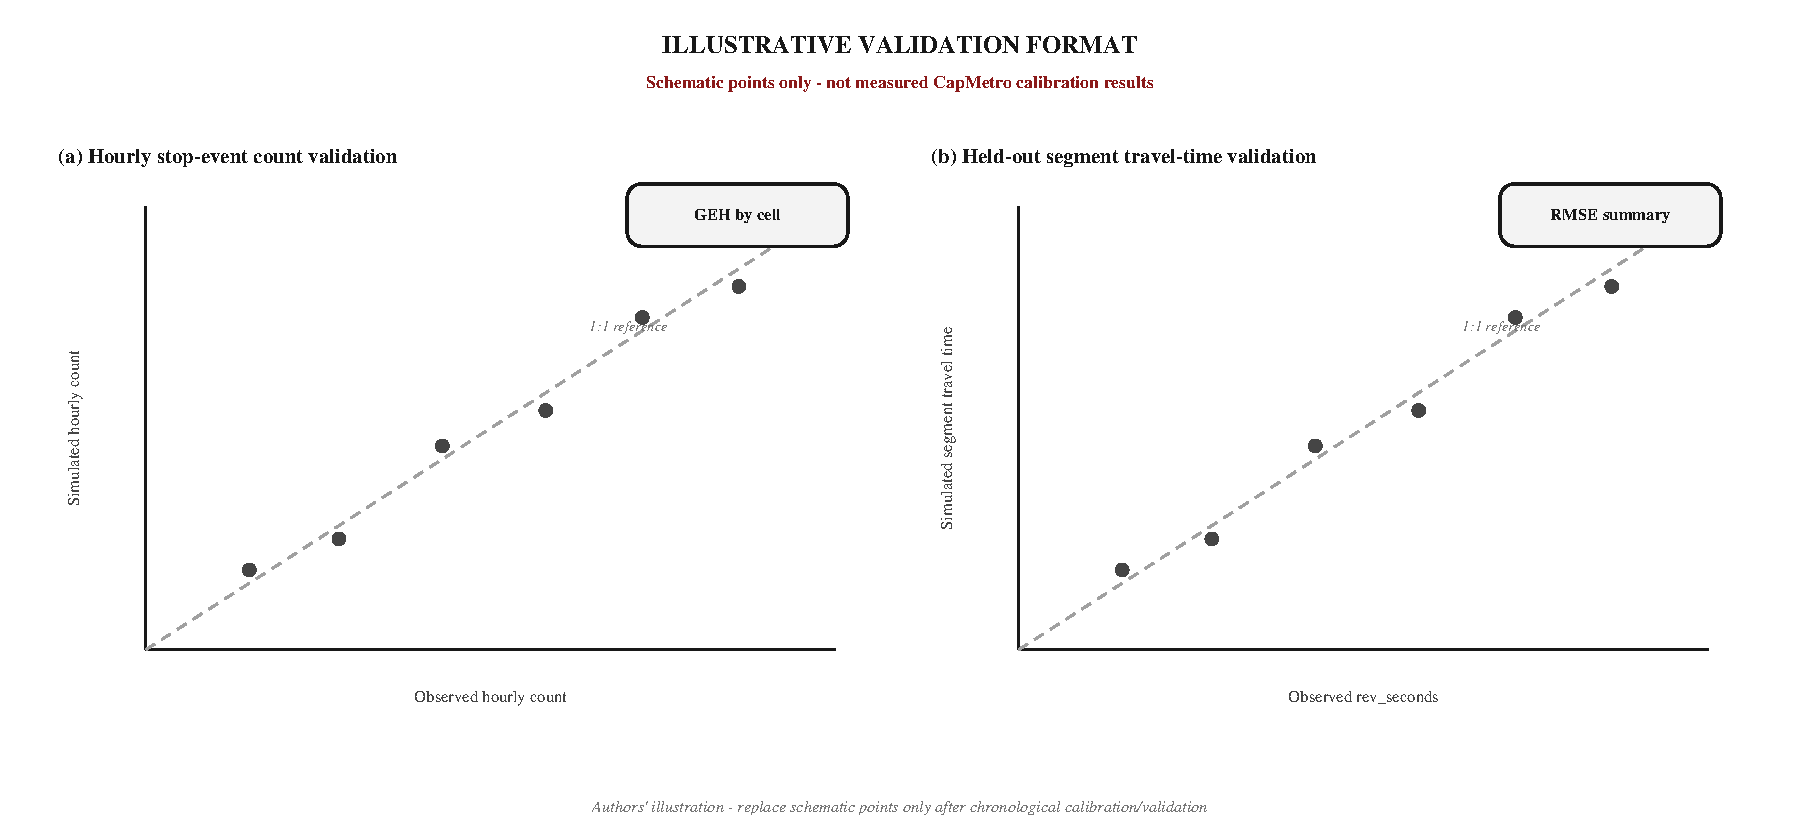
\includegraphics[width=\textwidth]{Figures/meth_fig_eo1_1_calibration (2).pdf}
    \caption[Illustrative SUMO calibration output]{Illustrative format of the
    SUMO calibration output. (a) GEH statistic for identically defined observed
    and simulated hourly stop-event counts. (b) Simulated segment travel time
    against held-out empirical \texttt{rev\_seconds} observations in the RMSE
    step. Values shown are illustrative only. Authors' illustration.}
    \label{fig:calibration-illustrative}
\end{figure}

\subsubsection{Bus Volume Validation via GEH Statistic}

The GEH statistic, introduced for traffic-modelling acceptance testing in the UK Design Manual for Roads and Bridges \cite{DMRBV12}, measures the discrepancy between simulated and observed hourly bus volumes on individual corridor segments, illustrated in panel (a) of Figure~\ref{fig:calibration-illustrative}:

\begin{equation} GEH = \sqrt{\frac{2(M - C)^2}{M + C}} \label{eq:geh} \end{equation}

where $M$ is the hourly bus volume from the simulation and $C$ is the observed hourly bus count from empirical operational data. The environment is accepted when $GEH < 5$ for more than 85\% of corridor segments, following the FHWA Traffic Analysis Toolbox calibration criterion~\cite{FHWA2019TAT} as applied in recent SUMO calibration work by Patil et al.~\cite{Patil2025Conformal}.

\subsubsection{Segment Travel-Time Calibration via RMSE}

Count calibration alone does not guarantee realistic movement. RMSE evaluates how closely simulated segment travel times match held-out empirical \texttt{rev\_seconds} observations, illustrated in panel (b) of Figure~\ref{fig:calibration-illustrative}:

\begin{equation} RMSE = \sqrt{\frac{\sum_{i=1}^{n}(x_{obs} - x_{model})^2}{n}} \label{eq:rmse} \end{equation}

where $x_{obs}$ is an observed segment travel time and $x_{model}$ is its simulated counterpart. Parameters such as desired speed and segment friction are tuned on the chronological calibration split, then evaluated once on the held-out split. A speed-based secondary RMSE is permitted only after distance units are verified. Until then, the travel-time measure is the reproducible calibration target.

\subsubsection{Real-Time Data Incorporation}

In a real-world deployment, forward and backward headways would come from AVL, onboard load from APC, waiting queues from AFC or platform sensing, and weather/incident flags from external services \cite{Wangsun}. In this study, APC data calibrate load, boarding, dwell, and segment travel-time distributions; NOAA data supply the observed ordinary-weather exposure; passenger arrival times, queues, and breakdown flags are generated by the simulation and are labeled accordingly.

\subsection{Operating Conditions}

The study uses five disturbance labels: baseline stochastic demand (D), demand surge (S), ordinary empirical travel-time variation (T), weather stress (W), and breakdown (B). D and T remain active in every training and evaluation run. This prevents the baseline from becoming deterministic and prevents W from replacing ordinary empirical travel-time variation.

\textbf{Training condition.} The policy is trained with D+T always active while S, W, and B are domain-randomized over their declared ranges. Weather exposure includes observed ordinary-rain strata where empirical support is adequate and labeled synthetic lognormal stress outside that support.

\textbf{Stage A baseline evaluation.} The frozen policy and all baseline controllers are evaluated under D+T, with S, W, and B disabled. This is an observed-data-calibrated stochastic baseline, not a claim of perfect or ``ideal'' real-world operation.

\textbf{Stage B combined-disturbance evaluation.} The frozen controllers are evaluated under D+T+S+W+B. Single-disturbance ablations add S only, W only, or B only to D+T. Consequently, ``weather-only'' denotes D+T+W and ``breakdown-only'' denotes D+T+B.

Table~\ref{tab:activation-matrix} is the authoritative activation matrix. A condition is an environment state; a baseline controller is an algorithmic comparator.

\begin{table}[htbp]
\centering
\caption{Authoritative disturbance-activation matrix.}
\label{tab:activation-matrix}
\small
\begin{tabularx}{\textwidth}{Xccccc}
\toprule
\textbf{Condition} & \textbf{D} & \textbf{T} & \textbf{S} & \textbf{W} & \textbf{B} \\
\midrule
Training & on & on & randomized & randomized & randomized \\
Stage A baseline & on & on & off & off & off \\
Stage B combined & on & on & on & on & on \\
S ablation & on & on & on & off & off \\
W ablation & on & on & off & on & off \\
B ablation & on & on & off & off & on \\
\bottomrule
\end{tabularx}
\end{table}

\begin{table}[htbp]
\centering
\caption{Simulation parameter summary: fixed, swept/variable, and derived parameters.}
\label{tab:sim-parameters}
\small
\renewcommand{\arraystretch}{1.25}

\begin{tabularx}{\textwidth}{
>{\RaggedRight\arraybackslash}p{0.24\textwidth}
>{\RaggedRight\arraybackslash}p{0.09\textwidth}
X
>{\RaggedRight\arraybackslash}p{0.20\textwidth}
}

\toprule
\textbf{Parameter} & \textbf{Symbol} & \textbf{Value / Range} & \textbf{Source} \\
\midrule
\multicolumn{4}{l}{\textit{Fixed simulation parameters}} \\
\midrule

Simulation horizon & --- & Single observed Route 801 service window (\texttt{\%TODO-DATA}: select start/end after historical schedule and timestamp-basis validation) & Section~3.1 \\
Total distinct stop IDs (direction code 6) & $M$ & 29 & Reproduced CapMetro APC audit \\
Fleet size (active buses) & $N$ & \%TODO-DATA: derive from concurrent Route 801 vehicle activity and verified schedule & CapMetro APC + historical GTFS \\
Control stop count & --- & \texttt{\%TODO-VAL}: select from 29 observed stop IDs using Section~3.2.2 criteria after calibration/validation & Section~3.2.2 \\
Scheduled headway & $H_0$ & \%TODO-DATA: 2021-compatible GTFS or schedule record & Historical CapMetro schedule \\
Bus passenger capacity & --- & \%TODO-DATA: verified vehicle/fleet specification & CapMetro fleet specification \\
Maximum holding duration & $\Delta T$ & \%TODO-VAL: to be set during implementation & Section~3.2.7 (Action Space) \\
Holding action bins & $\Omega$ & $\{0.0, 0.1, 0.2, 0.3, 0.4\}$ & Section~3.2.7 (Action Space) \\
Action space size per agent & $|A_i|$ & 10 (5 hold $\times$ 2 skip) & Section~3.2.7 (Action Space) \\
Monte Carlo runs per cell & $N_{\text{runs}}$ & $\geq 30$ & Section~3.1 \\
Discount / event-based discount & $\gamma$, $\beta$ & \%TODO-VAL: tuned during implementation & Section~3.2.7 \\

\midrule
\multicolumn{4}{l}{\textit{Swept / variable parameters}} \\
\midrule

Synthetic severe-weather intensity & $\eta$ & $\{0.0, 0.3, 0.6, 1.0, 1.3\}$; values above observed support are stress tests & Section~3.2.6 \\
Demand-surge scale & $f_d$ & $\mathcal{N}(1,\sigma_d^2)$ with \%TODO-VAL $\sigma_d$ and support clipped to $[1,3]$ & Section~3.2.6 \\
Traffic-speed stress scale & $f_s$ & $\mathcal{N}(1,\sigma_s^2)$ with \%TODO-VAL $\sigma_s$ and support clipped to $[0.8,1.2]$ & Section~3.2.6 \\
Breakdown rate & $\lambda$ & \texttt{\%TODO-VAL}: declared scenario rate (events per bus-hour); APC contains no failure events & Section~3.2.6 \\

\midrule
\multicolumn{4}{l}{\textit{Derived empirical/calibration parameters}} \\
\midrule

Baseline inter-stop travel time & $\mu$ & Per-segment, time-of-day, and day-type bin, to be computed & CapMetro \texttt{rev\_seconds} \\
Baseline travel-time std.\ dev.\ & $\sigma$ & Per-segment, time-of-day, and day-type bin, to be computed & CapMetro \texttt{rev\_seconds} \\
Baseline coefficient of variation & $CV_0$ & $\sigma/\mu$ per segment, \%TODO-DATA & Computed from dataset \\
Lognormal shape parameter & $\sigma_{ln}$ & $\sqrt{\ln(\eta^2+1)}$ (Eq.~\ref{eq:sigma_ln}) & Method of moments \\
Lognormal unit-mean factor location & $\mu_{ln}$ & $-\sigma_{ln}^2/2$ (Eq.~\ref{eq:mu_ln}) & Method of moments \\

\bottomrule
\end{tabularx}
\end{table}

Table~\ref{tab:sim-parameters} is the parameter reference for this chapter. A \texttt{\%TODO-VAL} is a design value still requiring an explicitly justified experimental choice; a \texttt{\%TODO-DATA} is a value blocked on an external source or unfinished empirical derivation. These visible RTC-compliant placeholders prevent unsupported target values from being mistaken for observed CapMetro quantities. The 29-stop count is reproduced from the clean direction-code 6 subset. The demand and speed clip supports are not standard deviations: $\sigma_d$ and $\sigma_s$ remain separate distribution parameters and cannot be replaced by their clip bounds.

\subsection{Data Processing}

The MARL framework is trained and evaluated on a single stream of input data pre-processed before training: corridor operational data used to calibrate SUMO and to derive baseline parameters for the stochastic generators. A second stream, the synthetic state observations generated by the Python environment at runtime, is produced on-the-fly during training and consumed once per control event.

\subsubsection{Required Datasets}

\begin{enumerate}
\item \textbf{CapMetro APC event data.} The official July--December 2021 Socrata asset \texttt{im6q-3pc9} contains 47 text-typed columns \cite{TexasCapMetroAPC2021}. The primary query keeps Route 801 records for which \texttt{current\_route\_id=route\_id}, \texttt{import\_error=0}, \texttt{import\_trip\_error=0}, \texttt{bs\_id}$\neq 0$, and \texttt{direction\_code\_id=6}. The checksum-recorded result contains 229{,}421 rows, 184 service-day codes, and 29 distinct stop IDs. It supplies event time, trip/vehicle keys, boardings, alightings, load, dwell, segment travel time/distance, coordinates, and quality flags.

\item \textbf{NOAA LCDv2 weather.} Camp Mabry (USW00013958) is the primary station and Austin-Bergstrom (USW00013904) is the sensitivity station \cite{NOAALCDv2}. NOAA timestamps are local standard time with no daylight-saving adjustment. They are interpreted as UTC$-06{:}00$, converted to \texttt{America/Chicago}, and joined to APC event time by nearest observation within 90 minutes. Both stations matched all 229{,}421 primary events in the feasibility audit; 11{,}804 events matched a Camp Mabry rain flag.

\item \textbf{Historical schedule and fleet metadata.} A 2021-compatible GTFS snapshot is required for authoritative direction labels, stop names, route shape, and scheduled headway; a verified fleet source is required for capacity. The current GTFS asset \cite{CapMetroGTFS} is not substituted for a historical snapshot. Until those gates close, direction 6 remains code-only and schedule/capacity parameters remain \%TODO-DATA.
\end{enumerate}

\begin{table}[htbp]
\centering
\caption{Verified CapMetro/NOAA fields and their modeling roles.}
\label{tab:field-mapping-texas}
\small
\renewcommand{\arraystretch}{1.2}
\begin{tabularx}{\textwidth}{p{0.25\textwidth}p{0.29\textwidth}X}
\toprule
\textbf{Source fields} & \textbf{Derived quantity} & \textbf{Model role and limitation} \\
\midrule
\texttt{apc\_date\_time}, \texttt{transit\_date\_time} & Event instant and service day & Chronological split and weather join; APC timezone remains a declared Austin-wall-clock assumption \\
\texttt{ext\_trip\_id}, \texttt{vehicle\_id}, \texttt{act\_trip\_start\_time}, \texttt{actual\_sequence} & Trip-day identity and event order & Headway/segment construction; no single field is assumed globally unique \\
\texttt{bs\_id}, direction code & Stop/segment sequence & 29 stop IDs for code 6; names and compass label require historical metadata \\
\texttt{ons}, \texttt{offs}, \texttt{max\_load} & Boarding, alighting, and load profiles & Demand/load calibration; not passenger arrival time or capacity \\
\texttt{dwell\_time} & Door-open to door-close seconds & Dwell distribution; controller holding is simulated separately \\
\texttt{rev\_seconds}, \texttt{rev\_distance} & Segment travel time and possible average speed & Travel-time RMSE is primary; distance unit remains unresolved \\
\texttt{veh\_lat}, \texttt{veh\_long}, \texttt{quality\_indicator} & Stop-event coordinates and GPS quality & Event-level QA; not a continuous trajectory \\
NOAA precipitation and present-weather code & Observed ordinary-rain flag & Primary weather exposure after time alignment \\
NOAA visibility, temperature, humidity, wind & Weather covariates & Controls/sensitivity variables, not primary exposure by default \\
\bottomrule
\end{tabularx}
\end{table}

Passenger arrival timestamps, waiting time, capacity, and breakdown events are absent from the APC file. They are simulated or separately sourced and are never described as directly observed. The pooled wet/dry travel-time medians produced by the feasibility audit are descriptive only; causal or calibration multipliers require segment, time-of-day, and day-type adjustment.

% Superseded EDSA/SafeTravelPH data plan retained inactive for source history.
\iffalse
\begin{itemize}

\item \textbf{Corridor bus operational data.} A per-trip record of EDSA Carousel bus operation along the study sub-corridor, collected over a continuous observation window of at least two weeks. The required fields are GPS-tracked vehicle location, boarding and alighting events, passenger occupancy, operating speed, and \textit{dwell time} at each stop, the dwell time being the interval a bus spends stationary at a stop serving passengers, measured from the moment the doors open to the moment they close and the bus is ready to depart, exclusive of any holding time subsequently imposed by the controller. These records yield the empirical distributions of bus cruising speed, inter-stop travel time, and demand under ideal operating conditions, used both to calibrate SUMO and to define the baseline operating point of the stochastic generators. The baseline operating point will be established only after the intended July 2023 SafeTravelPH EDSA Busway record has been acquired and its schema and coverage verified; no calibration or dataset-specific statistics are claimed at this stage.

%A crowdsourced operational dataset of this form, for example, data collected from the EDSA Busway via the SafeTravelPH mobile application, provides a representative model of the required structure. Should bus-volume coverage prove insufficient for the GEH validation step, supplementary records may be requested from MMDA, DOTr, or the involved bus operators under the Freedom of Information process.

\end{itemize}

Table~\ref{tab:field-mapping} maps each required raw field to the parameter derived from it and the MARL component that parameter feeds into, connecting the data requirements above to the disturbance generators (Section~\ref{subsec:stochastic-vars}), the control-stop selection criteria (Section~\ref{subsec:control-stop-selection}), and the agent observation vector (Section~\ref{subsec:state-space}). The mapping reflects the study's design intent, not properties of a processed dataset; specific statistics remain \%TODO-DATA pending dataset acquisition.

\begin{table}[htbp]
\centering
\caption{Mapping of required raw dataset fields to derived parameters and their role in the MARL formulation.}
\label{tab:field-mapping}
\small
\renewcommand{\arraystretch}{1.25}

\begin{tabularx}{\textwidth}{
>{\RaggedRight\arraybackslash}p{0.19\textwidth}
>{\RaggedRight\arraybackslash}p{0.28\textwidth}
>{\RaggedRight\arraybackslash}X
}

\toprule
\textbf{Raw Field} & \textbf{Derived Parameter} & \textbf{MARL Component} \\
\midrule

GPS-tracked vehicle location &
Per-segment inter-stop travel time distribution ($\mu$, $\sigma$) &
SUMO speed calibration (RMSE, Section~\ref{subsec:stochastic-vars}); anchors the traffic-speed generator ($\sigma_s$) and the weather generator's baseline mean ($\mu$) \\

Boarding events &
Per-(stop, time-of-day) baseline demand rate &
Demand surge generator baseline ($\sigma_d$); waiting-passenger-count feature in the agent's local observation \\

Alighting events &
Through-passenger volume per stop &
Control-stop selection criterion 3 (low through-volume preference, Section~\ref{subsec:control-stop-selection}) \\

Passenger occupancy &
Per-segment load profile &
Onboard-passenger-count feature in the agent's local observation; dwell-time estimation \\

Operating speed &
Per-segment baseline cruising speed &
SUMO bus-volume calibration (GEH); traffic-speed generator baseline ($\sigma_s$) \\

Dwell time &
Per-(stop, time-of-day) dwell time distribution &
Event-driven bus model, used between control events to advance the simulation clock \\

\bottomrule
\end{tabularx}
\end{table}

Severe-weather conditions are not estimated from operational data in this study but are injected as a controlled experimental variable, with disturbance magnitudes anchored to validated literature values rather than to a corridor-specific severe-weather sample.

A short empirical observation window cannot reliably resolve the variance of a heavy-tailed severe-weather distribution at per-segment granularity, and a swept-disturbance design characterizes controller performance across a range of conditions rather than at a single uncertain calibration point. Because the disturbance conditions are random by construction, they are not drawn from any single fixed dataset: each Monte Carlo run generates a fresh, independently seeded realization of demand, traffic-speed, weather, and breakdown disturbances. The single empirical dataset is required only to fix the \textit{baseline} (ideal-condition) operating point against which these random disturbances are layered; the held-out validation split (Stage 3 below) confirms that the calibrated baseline generalizes beyond the records used to tune it. The full disturbance parameterization is described in Section~\ref{subsec:stochastic-vars}.

\fi
\subsubsection{Data Pre-Processing Pipeline}
\label{subsec:data-pipeline}

Pre-processing proceeds in three stages.

\textit{Stage 1: acquisition, integrity, and time normalization.} The pipeline records the Socrata query, row count, 47-field schema, file size, and SHA-256 hash. It applies the declared route/error/stop/direction filters before modeling. APC compact timestamps are parsed as Austin wall-clock time; NOAA LCDv2 local-standard timestamps are assigned fixed UTC$-06{:}00$ and converted to \texttt{America/Chicago}. Ambiguous fall-back APC times are counted and assigned a declared fold rather than silently duplicated. Records with invalid timestamps or non-positive segment time/distance are excluded only from the derivation that requires those values, not from unrelated demand/dwell summaries.

\textit{Stage 2: sequence construction and empirical extraction.} Events are ordered using service day, trip/vehicle keys, actual trip start, and actual sequence. Per-(stop, time-of-day, day-type) boarding, alighting, load, and dwell distributions are estimated. Per-(segment, time-of-day, day-type) \texttt{rev\_seconds} distributions yield $\mu$, $\sigma$, and $CV_0$. Because the source spans 184 service-day codes, weekday/weekend and time-bin support is assessed empirically rather than assuming a two-week window.

\textit{Stage 3: weather alignment and controlled estimation.} Each APC event is assigned the nearest Camp Mabry observation within 90 minutes and a Bergstrom sensitivity match. Primary exposure uses precipitation and present-weather rain codes; visibility is secondary, and temperature, humidity, and wind are candidate controls. Any ordinary-rain multiplier is estimated within segment, time-of-day, and day-type strata. The unadjusted pooled wet/dry difference is not used as a causal multiplier.

\textit{Stage 4: chronological calibration/validation split.} Earlier service days tune SUMO and the empirical parameter files; later held-out days assess stop-event counts and segment travel-time RMSE. No held-out record is used to choose calibration parameters.

The MARL agents are not trained on these raw datasets directly. They are trained on synthetic state vectors $s_{i,t}$ produced by the Python environment at each control event. Each $s_{i,t}$ is assembled at runtime by querying the analytical bus model and is consumed once by the policy network before being discarded. There is no persistent training dataset of state-action transitions on disk other than the standard replay buffer used by the learning algorithm.

\subsection{Stochastic Disturbance Generators}
\label{subsec:stochastic-vars}

\paragraph{Disturbance Classes and Independence}

This study distinguishes five disturbance classes, denoted D, S, T, W, and B:

\begin{itemize}
\item \textbf{Stochastic demand (D):} represents the normal day-to-day variation in passenger arrivals. Passenger demand is sampled from calibrated distributions for each stop and time of day (Section~\ref{subsec:data-pipeline}). Unlike the other disturbances, D is always active and serves as the baseline demand condition of the simulation rather than an additional disturbance applied to a fixed demand profile.
\item \textbf{Demand surge (S):} represents an increase in passenger demand by scaling the baseline boarding rates for a given episode, with standard deviation $\sigma_d$ (Table~\ref{tab:notation}). In this case, D remains active as the baseline demand variation, while S introduces an additional increase in demand. Setting $\sigma_d = 0$ removes the surge and leaves only the baseline stochastic demand represented by D.
\item \textbf{Ordinary travel-time variation (T):} the always-present empirical per-(segment, time-of-day, day-type) distribution derived from \texttt{rev\_seconds}. An optional episode-level stress scale $f_s$ may broaden this baseline, with its standard deviation $\sigma_s$ selected separately from the $[0.8,1.2]$ clip support.
\item \textbf{Weather-induced delay (W):} an additive experimental layer. Within observed support, W is estimated by comparing rain-exposed and dry observations within segment/time/day strata. Outside that support, W is a labeled synthetic lognormal stress with coefficient of variation $\eta$. W composes with rather than replaces T.
\item \textbf{Discrete bus breakdown (B):} represents the occurrence of bus breakdowns during operation. Breakdowns are modeled as discrete events following a Poisson distribution with rate $\lambda$. Once a bus breaks down, it is removed from the active fleet for the remainder of the simulated day.
\end{itemize}

The generators for S, W, and B are sampled independently while D and T serve as the baseline conditions. Therefore, one disturbance does not directly trigger another within the simulation: a bus breakdown does not cause a demand surge or weather delay, and weather conditions do not cause a bus breakdown. This setup allows the individual effect of each disturbance to be evaluated more clearly during the single-disturbance ablation experiments. However, this assumption is only used for the simulation design and does not imply that these disturbances are necessarily independent in real-world operations.

Four stochastic generators inject variability into the Python environment. Generators (i) and (ii) follow the perturbation framework of Wang and Sun~\cite{Wangsun}; the weather generator's heavy-tailed lognormal formulation follows Patil et al.~\cite{Patil2025Conformal}; the breakdown generator follows the rescheduling formulation of Cao et al.~\cite{Cao2022Train}. Table~\ref{tab:notation} collects the symbols used across this section and the MARL formulation that follows.


\begin{table}[htbp]
\centering
\caption{Notation used in the stochastic generators and the MARL formulation.}
\label{tab:notation}

\small
\renewcommand{\arraystretch}{1.25}

\begin{tabularx}{\textwidth}{
>{\RaggedRight\arraybackslash}p{0.14\textwidth}
>{\RaggedRight\arraybackslash}X
>{\RaggedRight\arraybackslash}p{0.18\textwidth}
}

\toprule
\textbf{Symbol} & \textbf{Definition} & \textbf{Domain / units} \\
\midrule

$\eta$ &
Synthetic out-of-support weather-stress intensity; sets the coefficient of variation of the added lognormal travel-time stress. $\eta=0$ disables this synthetic layer. &
dimensionless \\

$\sigma_d$ &
Standard deviation of the per-episode passenger-demand scaling factor. $\sigma_d=0$ fixes demand at its baseline mean. &
dimensionless \\

$\sigma_s$ &
Standard deviation of the per-episode traffic-speed scaling factor. $\sigma_s=0$ fixes cruising speed at its baseline mean. &
dimensionless \\

$\lambda$ &
Rate parameter of the Poisson process governing bus breakdowns. $\lambda=0$ disables breakdowns. &
events/hour \\

$\mu$ &
Baseline (empirical) mean inter-stop travel time for a given segment and time-of-day bin. &
seconds \\

$\sigma$ &
Baseline standard deviation of inter-stop travel time. &
seconds \\

$CV_0$ &
Baseline coefficient of variation, $CV_0=\sigma/\mu$, used to anchor the disturbance generators. &
dimensionless \\

$\mu_{ln},\sigma_{ln}$ &
Location and shape parameters of the lognormal weather-delay distribution (method-of-moments). &
--- \\

$h^-,\hat{h}^+$ &
Forward headway (gap to bus ahead) and estimated backward headway (gap to bus behind). &
seconds \\

$H_0$ &
Desired (scheduled) headway. &
seconds \\

$\alpha_{i,t}$ &
Holding-strength action of agent $i$, $\alpha_{i,t}\in\Omega=\{0.0,0.1,0.2,0.3,0.4\}$, scaled by $\Delta T$. &
dimensionless \\

$\Delta T$ &
Maximum holding duration that $\alpha_{i,t}$ scales. &
seconds \\

$\gamma,\beta$ &
Discount factor and event-based discount rate ($e^{-\beta t}$ replaces $\gamma$ for random inter-event times). &
dimensionless \\

$\theta$ &
Weights (parameters) of the online neural network (shared policy). &
dimensionless \\

$\theta^-$ &
Weights (parameters) of the target neural network in DDQN. &
dimensionless \\

$N$ &
Number of active bus agents. &
count \\

$N_{\mathrm{runs}}$ &
Number of independent Monte Carlo replications per controller/condition cell. &
count \\

\bottomrule
\end{tabularx}
\end{table}

\subsubsection{Random Seed Control}

A stored master seed initializes named NumPy child streams for D, S, T, W, B, passenger arrivals, and policy exploration. Separating streams ensures that enabling W does not shift the random draws assigned to demand or breakdowns. Within an evaluation cell, the same master-seed list and generator substreams are reused across all four controllers, so run $k$ is a matched counterfactual comparison \cite{Henderson2018Matters}. Seeds differ across replications. The minimum $N_{\mathrm{runs}}\geq30$ does not replace distribution diagnostics; bootstrap intervals are used for heavy-tailed responses \cite{Agarwal2021Precipice}.

\subsubsection{Passenger Demand}

The baseline empirical transit demand is adjusted at each episode using a scaling factor sampled from $\mathcal{N}(1, \sigma_d^2)$ and clipped to $[1, 3]$. This follows the general Gaussian-clipped demand-scaling approach used by Wang and Sun~\cite{Wangsun}, but this study uses a narrower range than their $[1, 10]$ setting. The asymmetric range focuses the experiments on demand surges rather than demand reductions, since lower demand mainly produces lightly loaded conditions and does not provide the same level of stress on the controller. The upper bound of 3, which allows the baseline boarding rate to increase by roughly three times, is a choice specific to this study (\%TODO-VAL: revisit against Wang and Sun's wider range during implementation) rather than a value directly adopted from prior work. Sampling occurs at the start of each simulation run, producing varied demand profiles across episodes. In implementation, the scaling factor $f_d \sim \mathcal{N}(1, \sigma_d^2)$ is sampled once per episode at initialization and applied uniformly to every per-stop, per-time-of-day arrival rate for the duration of that simulated operating day, so all stops experience the same proportional demand shift within a single run while the shift itself varies across runs.

\subsubsection{Traffic Delays}

Ordinary inter-stop travel time is sampled from the empirical T distribution for the current segment, time-of-day, and day-type stratum. If a separate corridor-wide stress test is retained, $f_s \sim \mathcal{N}(1,\sigma_s^2)$ is sampled once per episode and clipped to $[0.8,1.2]$ \cite{Wangsun}; $\sigma_s$ is a \%TODO-VAL and is not equal to either clip bound. T remains active when W or B is enabled. Thus a weather run preserves ordinary empirical variability and applies its weather layer on top, avoiding the previous replacement/double-definition conflict.

\subsubsection{Weather-Induced Anomalies}

The weather design has two explicitly separated layers. \textbf{Observed ordinary weather} uses the timestamp-aligned NOAA records. Rain exposure is defined primarily from precipitation and present-weather rain codes at Camp Mabry, with Austin-Bergstrom as a sensitivity station. For each segment/time-of-day/day-type stratum with adequate wet and dry support, the implementation estimates a regularized multiplier $m_{s,b,d}(w)$ relative to its dry baseline. Temperature, humidity, wind, and visibility may enter the estimation as controls. No pooled wet/dry median is used as a causal multiplier.

\textbf{Synthetic severe/extreme weather} is used only outside the support of the observed strata. It applies a unit-mean lognormal factor $F_W$ to a draw $T_0$ from the always-active empirical T distribution. This preserves the ordinary segment variation instead of replacing it:

\begin{equation}
T_W = T_0\,m_{s,b,d}(w)\,F_W.
\label{eq:weather-compose}
\end{equation}

For an exclusively synthetic stress cell, $m_{s,b,d}(w)=1$. The controlled parameter $\eta$ is the coefficient of variation of $F_W$, not a rainfall intensity or a named meteorological category. The lognormal form represents right-skewed travel-time stress and follows the distributional rationale of Patil et al.~\cite{Patil2025Conformal}:

\begin{equation} CV = \eta \label{eq:cv_eta} \end{equation}

The lognormal shape and scale parameters follow the method-of-moments derivation:

\begin{equation} \sigma_{ln} = \sqrt{\ln(\eta^2 + 1)} \label{eq:sigma_ln} \end{equation}

\begin{equation} \mu_{ln} = -\frac{\sigma_{ln}^2}{2} \label{eq:mu_ln} \end{equation}

The factor is drawn as $F_W \sim \text{LogNormal}(\mu_{ln},\sigma_{ln})$, for which Equations~\eqref{eq:sigma_ln}--\eqref{eq:mu_ln} give $\mathbb{E}[F_W]=1$ and $CV(F_W)=\eta$. Patil et al.~\cite{Patil2025Conformal} validate a CV-driven lognormal travel-time form against SUMO/INRIX-based urban arterial scenarios. This study uses that form for a declared extrapolative stress factor; it does not claim that Patil et al.'s CV values correspond to Austin rainfall categories.

The synthetic factor is swept over $\eta \in \{0.0,0.3,0.6,1.0,1.3\}$. Values through 1.0 span the range evaluated by Patil et al.; 1.3 is a deliberate extrapolation. None is assigned a rain-rate label. Observed ordinary-rain experiments are reported by their NOAA exposure definition rather than by $\eta$.

\begin{table}[htbp]
\centering
\caption{Basis for each synthetic weather-stress intensity value.}
\label{tab:eta-basis}
\small
\renewcommand{\arraystretch}{1.25}

\begin{tabularx}{\textwidth}{
>{\Centering\arraybackslash}p{0.08\textwidth}
X
}

\toprule
\textbf{$\eta$} & \textbf{Basis} \\
\midrule

0.0 & Synthetic factor off; empirical T remains active \\
0.3 & Within the published CV range; synthetic variability stress \\
0.6 & Within the published CV span; synthetic variability stress \\
1.0 & Upper end of the published CV range; synthetic severe stress \\
1.3 & Beyond the published range; deliberate extreme extrapolation \\

\bottomrule
\end{tabularx}
\end{table}

The mapping from $\eta$ to named weather severity is not established. The sweep is reported as synthetic travel-time variability, whereas ordinary rain is evaluated through the empirical NOAA join. Keeping the two layers separate prevents observed rain, literature-shaped stress, and out-of-range extrapolation from being presented as one calibrated variable.

\subsubsection{Bus Breakdowns}

Unlike the perturbations above, a bus breakdown is a \textit{discrete event} that removes a vehicle from active simulation. Cao et al.~\cite{Cao2022Train} model Poisson train malfunctions in an adjacent MARL rescheduling setting, while Guedes and Borenstein~\cite{Guedes2018Rescheduling} model serious public-transit vehicle failures in heuristic real-time rescheduling. These sources support the event/removal semantics, not an empirical CapMetro failure rate; the APC data contain no breakdown field. Breakdowns are therefore a labeled synthetic stressor triggered at random times from a Poisson process with a configurable scenario rate $\lambda$ (Table~\ref{tab:notation}). In implementation, at each discrete simulation timestep of length $dt$, a Bernoulli trial with probability $\lambda \cdot dt$ is evaluated independently for each active bus; a success removes that bus from the active agent set for the remainder of the simulated day. When a breakdown occurs at bus $b_k$, $b_k$ is removed from the active agent set, leaving an enlarged headway between the trailing bus $b_{k-1}$ and the leading bus $b_{k+1}$. The passengers that $b_k$ would have served accumulate at the stops ahead of $b_{k-1}$, so the trailing bus inherits this residual demand as it advances.

A breakdown does not override any surviving agent's policy; it changes the state and reward landscape. Removing $b_k$ enlarges the gap between the trailing and leading buses, and passengers that would have boarded $b_k$ continue accumulating in the simulated queues. A trailing agent may choose to hold less or skip a stop to close the gap, but a skipped stop serves neither boarding nor alighting passengers in that event and therefore incurs the waiting/skip penalty. The environment never injects a recovery action: every hold/skip decision originates from $\pi_\theta$.

The Poisson assumption is a tractable approximation for the single-day simulation horizon, over which vehicle age, maintenance schedule, and mileage since last service can be treated as constant.


\subsection{MARL Architecture and MDP Formulation}

This subsection builds the formal learning framework in two steps. It first introduces the Bellman recursion that underlies value-based reinforcement learning, then specifies the Markov game tuple, the per-agent observation and action spaces, the reward-function design, and the proposed learning algorithm. The justification for choosing a multi-agent formulation over a single-agent alternative is presented in Chapter~1.

\subsubsection{Bellman Foundation}

At the core of reinforcement learning is the dynamic programming principle established by Bellman~\cite{Bellman1957}. The agent's objective is to maximize the expected sum of discounted future rewards. The state-action value function $Q^\pi(s,a)$, denoting the expected return from taking action $a$ in state $s$ and following policy $\pi$ thereafter, satisfies the Bellman optimality equation:

\begin{equation}
Q^*(s, a) = \mathbb{E} \left[ r(s, a) + \gamma \max_{a'} Q^*(s', a') \mid s, a \right]
\label{eq:bellman}
\end{equation}

where $s'$ is the state reached after applying action $a$, $r(s,a)$ is the immediate reward, and $\gamma \in [0, 1)$ is the discount factor. This equation is relevant here for two reasons. First, it shows that a long-horizon control policy can be learned by recursively backing up local one-step rewards, making it computationally feasible to evaluate the downstream effects of a holding or skipping decision without enumerating every future stop on the route. Second, in the asynchronous bus-control setting, the time between two consecutive control events is itself random. Following Bradtke and Duff~\cite{Bradtke1995}, the discount factor in Eq.~\eqref{eq:bellman} is replaced by an event-based discount $e^{-\beta t}$ that scales with the elapsed time between events. Each agent's learning target is therefore an event-adjusted version of Eq.~\eqref{eq:bellman}, not a fixed-tick MDP target. By convention throughout this chapter, $\gamma$ denotes the nominal discount factor as it appears in the canonical Bellman and DDQN equations, while $e^{-\beta t}$ is the event-based discount actually applied in the asynchronous setting; wherever $\gamma$ appears in a value-function equation, it is instantiated by $e^{-\beta t}$ at runtime.


\subsubsection{Markov Game Formulation}

Following Littman~\cite{Littman1994}, the bus fleet control problem is formulated as a multi-agent extension of a Markov Decision Process, a Markov game defined by the tuple $G = \langle N, S, A, P, R, \gamma \rangle$:

\begin{itemize}
\item $N$: number of bus agents.
\item $S$: joint state space.
\item $A$: joint action space.
\item $P$: state-transition function $P(s_{t+1}\mid s_t, a_t)$.
\item $R$: reward function.
\item $\gamma \in [0, 1)$: discount factor.
\end{itemize}

Because bus control is asynchronous and event-driven, agents act only upon arrival at a control stop. The formulation maintains a per-agent local transition $P_i : S_i \times A_i \rightarrow S_i$, with $S_i$ the local observation of agent $i$ \cite{Wangsun,Rodriguez2023Cooperative}.

\subsubsection{Agents ($N$)}

The decision-making agents are the individual bus units $i \in N$ operating along the corridor. To avoid combinatorial blow-up and to keep the system invariant to fleet size, all agents share a single neural-network policy under a \textbf{parameter-sharing} architecture and act on their own local observations at deployment \cite{Wangsun,Rodriguez2023Cooperative,Christianos2021PS}. Parameter sharing means that one set of network weights serves every bus; each bus computes its own action from its own observation, but learning updates from any bus improve the policy for all.

\subsubsection{State Space and Local Observations ($S_i$)}
\label{subsec:state-space}

The local observation $s_{i,t}$ at agent $i$ on arrival at a control stop is a vector composed of:

\begin{itemize}
\item \textbf{Spatial location:} index of the current control stop.
\item \textbf{System regularity:} forward headway $h^-$ and estimated backward headway $\hat{h}^+$, both available from AVL feeds in deployment \cite{Wangsun}.
\item \textbf{Passenger demand:} onboard passenger count and estimated number of passengers waiting at the stop, available from APC/AFC systems \cite{Wangsun}.
\item \textbf{Environmental flags:} encoded indicators for the current disturbance intensity and any active downstream incident or breakdown.
\end{itemize}

\begin{table}[htbp]
\centering
\caption{Agent observation vector: features, symbols, and data sources.}
\label{tab:observation-features}
\small
\renewcommand{\arraystretch}{1.25}

\begin{tabularx}{\textwidth}{
>{\RaggedRight\arraybackslash}p{0.24\textwidth}
>{\RaggedRight\arraybackslash}p{0.11\textwidth}
>{\RaggedRight\arraybackslash}X
>{\RaggedRight\arraybackslash}X
}

\toprule
\textbf{Feature} & \textbf{Symbol} & \textbf{Deployment Source} & \textbf{Simulation Source} \\
\midrule

Control stop index & --- & Route map (static) & Hardcoded stop list \\
Forward headway & $h^-$ & AVL feed & Event-driven bus model \\
Estimated backward headway & $\hat{h}^+$ & AVL feed & Event-driven bus model \\
Onboard passenger count & --- & APC system & Running tally in bus model \\
Waiting passenger count at stop & --- & AFC terminal / platform sensors & Simulated stop queue; not an APC field \\
Weather exposure/stress flag & $w$ (encoded) & Weather API / public incident alert & Joined NOAA exposure or labeled synthetic W parameter \\
Downstream incident / breakdown flag & $b$ (binary) & Incident management system & Breakdown generator output \\

\bottomrule
\end{tabularx}
\end{table}

As Table~\ref{tab:observation-features} shows, the environment generates each runtime observation from its evolving simulated state. Empirical APC/NOAA records calibrate the distributions and exposure strata before training; raw sensor rows are not streamed into the policy during an episode.

\subsubsection{Action Space ($A_i$)}
\label{subsec:action-space}

The agent's action $a_{i,t} = \pi_\theta(s_{i,t})$ combines two discrete components, following Rodriguez et al.~\cite{Rodriguez2023Cooperative}:

\begin{itemize}
\item \textbf{Holding control:} a holding-strength parameter $\alpha_{i,t} \in \Omega = \{0.0, 0.1, 0.2, 0.3, 0.4\}$, multiplied by a maximum holding duration $\Delta T$ to yield seconds held; $\alpha_{i,t} = 0$ means no holding.
\item \textbf{Stop-skipping:} a binary decision to bypass the next stop, allowing headway recovery at an explicit passenger-service cost. The policy chooses the action from local delay, load, and queue state; no capacity threshold is assumed until vehicle capacity is verified. Skipping is disallowed at the origin terminal and is not permitted if the immediately preceding trip already skipped that stop, so no stop is skipped by two consecutive trips.
\end{itemize}

This study uses an action space consisting of $|A_i| = 5 \times 2 = 10$ discrete actions, combining five holding strengths with two skip choices that can be selected independently. This provides a broader action space compared with the combined holding-and-skipping controller used by Rodriguez et al.~\cite{Rodriguez2023Cooperative}, which consists of six mutually exclusive actions: five holding strengths $\Omega = \{0.0, 0.1, 0.2, 0.3, 0.4\}$, where zero holding already represents the option of not holding, and one separate skip action. Both studies use the same five-value set for holding strength.

A continuous holding parameter $\alpha \in [0, 1]$ was considered but was not used for two main reasons. First, continuous actions generally require actor-critic algorithms, which can introduce additional training instability. Second, continuous precision is not necessarily meaningful during actual deployment because driver compliance with holding instructions is imperfect. Rodriguez et al.~\cite{Rodriguez2023Cooperative} account for this by modeling non-compliant drivers as executing only 60--80\% of the instructed holding time. Therefore, using a continuous holding value would provide a level of control precision that may not be reliably achieved in practice.

\subsubsection{Reward Function ($R$) and Objective}
\label{subsec:reward}

The infinite-horizon objective of agent $i$ is the expected cumulative event-discounted return

\begin{equation}
R_i = \mathbb{E}\!\left[\sum_{k=0}^{\infty} e^{-\beta t_k}\, r_{i, t+k}\right],
\end{equation}

where $t_k$ is the elapsed time to the $k$-th future control event, consistent with the event-based discount introduced earlier.

The \textbf{structure} of the per-event reward $r_{i, t+k}$ --- its component terms and the operational priorities they encode --- is defined in this chapter. Its \textbf{exact weighting and sensitivity analysis} are a research objective of this study (Specific Objective 2, Expected Output 2.1), to be finalized during implementation rather than inherited from prior work. This separation is deliberate: the reward \textit{form} is grounded here, while the tuning of its coefficients is treated as an empirical question. The reward formulation must balance three competing operational priorities: (i) headway regularity, since bunching is the primary failure mode of bus corridors; (ii) passenger waiting time at served stops, which is the most direct passenger-experience metric; and (iii) a penalty term that discourages degenerate skipping behavior, since an unconstrained skip action could otherwise reduce headway variance by refusing to serve passengers. Existing MARL bus-control reward formulations span a range of trade-offs among these priorities, from headway-coefficient-of-variation forms for holding-only action spaces \cite{Wangsun,Wang2023MultiObj} to passenger-time forms for combined holding-and-skipping action spaces \cite{Rodriguez2023Cooperative}. This study defines the reward structure for the hybrid action space using the three component terms described above. The overall structure of the reward is fixed, while the relative weights of the three components, together with their sensitivity analysis, will be finalized during the implementation phase as part of Expected Output 2.1. The coefficients are therefore treated as placeholders at this stage.

The reward is computed individually for each agent at every control event rather than using a shared team-level reward. The value $r_{i,t}$ represents the reward assigned to agent $i$ in the transition tuple stored in the shared replay buffer (Training and Execution Protocol, step 4). This means that each bus is evaluated based on the consequences of its own action, even though all agents use the same shared network for learning. Since the agents already observe locally available quantities, particularly the forward and backward headway components, the individual reward can still capture the effects of an agent's action on corridor-wide regularity without requiring a centralized reward calculation during execution.

The three priorities are combined as a weighted sum of per-event penalty terms:

\begin{equation}
r_{i,t+k} = -w_1 \cdot (\text{headway-irregularity term}) - w_2 \cdot (\text{waiting-time term}) - w_3 \cdot (\text{skip-degeneracy term}),
\label{eq:reward-form}
\end{equation}

The weights $w_1$, $w_2$, and $w_3$ are left as placeholders (\%TODO-VAL) and will be tuned through the Expected Output 2.1 sensitivity analysis. Each component is expressed as a non-positive penalty, allowing the agent to maximize its expected return in Eq.~\eqref{eq:bellman} by minimizing headway irregularity, passenger waiting time, and excessive or degenerate skipping. Therefore, what is fixed in this chapter is the overall reward structure and its sign convention, while the specific component formulas and relative weights will be finalized during implementation.

\subsubsection{Proposed Learning Algorithm}
\label{subsec:proposed-algorithm}

The fully discrete action space ($|A_i| = 10$) makes value-based learning a natural fit. This study adopts \textbf{Double Deep Q-Network (DDQN)~\cite{vanHasselt2016DDQN} with parameter sharing under centralized training and decentralized execution (CTDE)}. Centralization here means that one learner samples per-agent local transitions from a shared replay buffer and updates one shared online/target network. It does not mean that the DDQN actor consumes a joint state or shared team reward: each transition contains agent $i$'s local observation and per-agent reward during both training and execution. The choice follows Rodriguez et al.~\cite{Rodriguez2023Cooperative}, who used a DDQN-based framework for cooperative holding-and-skipping control on a comparable corridor.

DDQN is chosen over three categories of alternatives. \textit{Plain DQN}~\cite{Mnih2015DQN} overestimates Q-values in noisy environments \cite{vanHasselt2016DDQN,Henderson2018Matters}, which the high-variance disturbance regime in this study would amplify. DDQN's double estimator addresses this by decoupling action selection from evaluation \cite{vanHasselt2016DDQN}. \textit{Actor-critic methods such as MAPPO and MADDPG} are compatible with continuous action spaces but unnecessary given the discrete action-space decision above; they would also introduce training instability that compounds across the swept-disturbance evaluation budget. \textit{Distributional methods such as Wang and Sun's IQNC-M} \cite{Wangsun} model the full return distribution rather than its expectation and offer strong performance on this problem class, but their meta-learning training procedure adds implementation risk beyond the scope of a thesis-scale project; IQNC-M is noted as a comparison target for future work.

Two enhancements from the recent bus-control literature will be tested during implementation: extending agent awareness to include neighboring-trip information in the observation and reward, as in Rodriguez et al.'s DDQN-HA variant \cite{Rodriguez2023Cooperative}, and credit assignment via inductive graph learning, as in Wang and Sun's CAAC framework \cite{Wangsun}. The final architecture will be selected based on training stability and validation-set passenger waiting time after a fixed training budget.


\subsubsection{Double Deep Q-Network Foundation}
\label{subsec:ddqn-foundation}

The Bellman optimality equation defines the value $Q^*(s,a)$ that an ideal controller would assign to each state-action pair, but it cannot be solved exactly for a state space as large as the bus-control problem, where the observation is a continuous vector of headways, loads, and queues. Two approximations bridge this gap. $Q$-learning~\cite{Bellman1957,Littman1994} replaces the exact solution with an iterative update that nudges a stored estimate $Q(s,a)$ toward the one-step Bellman target $r + \gamma \max_{a'} Q(s',a')$ after each transition. The Deep $Q$-Network (DQN)~\cite{Mnih2015DQN} replaces the lookup table with a neural network $Q(s,a;\theta)$, so that the value function generalizes across the continuous state vectors the bus environment produces. DQN trains $\theta$ by minimizing the temporal-difference loss between the network's prediction and a target computed from a periodically frozen copy of the network, with transitions drawn from an experience replay buffer to decorrelate consecutive samples.

DQN has a known issue: it systematically overestimates action values~\cite{vanHasselt2016DDQN}. The cause is the single $\max$ operator in the target. Because the same network both selects the next action ($\arg\max_{a'}$) and evaluates it ($\max_{a'} Q$), noise in value estimates is amplified the $\max$ preferentially picks whichever action happens to be overvalued, and that inflated value propagates into the target. In a low-variance environment this bias is manageable, but the swept-disturbance regime in this study generates heavy-tailed returns that feed the overestimation mechanism directly.

The Double Deep $Q$-Network (DDQN)~\cite{vanHasselt2016DDQN} removes this bias by decoupling action selection from action evaluation. The online network (weights $\theta$) selects the next action, but a separate target network (weights $\theta^-$) evaluates that action's value:

\begin{equation}
y^{\text{DDQN}} = r(s,a) + \gamma\, Q\!\left(s',\, \arg\max_{a'} Q(s', a'; \theta);\; \theta^-\right),
\label{eq:ddqn_target}
\end{equation}

For the overestimation to persist, both networks would have to overvalue the same action simultaneously, which is less likely than a single network doing so alone. The network is trained by minimizing the squared temporal-difference error:

\begin{equation}
\mathcal{L}(\theta) = \mathbb{E}_{(s,a,r,s') \sim \mathcal{D}} \left[ \left( y^{\text{DDQN}} - Q(s,a;\theta) \right)^2 \right],
\label{eq:ddqn_loss}
\end{equation}

where $\mathcal{D}$ is the experience replay buffer and the target weights $\theta^-$ are held fixed for a number of updates (or slowly tracked toward $\theta$) so that the regression target does not shift at every step.

Three properties make DDQN appropriate for this study. First, the discrete action space ($|A_i| = 10$) is the setting value-based methods handle well: the $\arg\max$ in Eq.~\eqref{eq:ddqn_target} is a finite enumeration over ten options. Second, the double estimator addresses the overestimation that high-variance disturbance returns would otherwise amplify. Third, DDQN inherits DQN's experience-replay and target-network machinery, which provides sufficient training stability without the auxiliary mechanisms that actor-critic methods require; this point is discussed further in Section~\ref{sec:challenges}. The event-based discount $e^{-\beta t}$ replaces the fixed $\gamma$ in Eq.~\eqref{eq:ddqn_target} when the target is computed in the asynchronous setting, so the DDQN target inherits the same event-adjustment as the underlying Bellman recursion. The combination of DDQN with parameter sharing and the CTDE scheme is specified in the Proposed Learning Algorithm subsection.

\subsubsection{Training and Execution Protocol}

The learning process follows the standard reinforcement-learning feedback loop under the asynchronous, event-driven bus-control setting and the CTDE scheme described above, illustrated in Figure~\ref{fig:aec-training}. The loop, repeated at every control event during training, proceeds as follows:

\begin{enumerate}
\item \textbf{Observe.} When bus agent $i$ arrives at a control stop, the Python environment assembles its local observation $s_{i,t}$ (Section~\ref{subsec:state-space}) from the analytical bus model and the active stochastic generators.
\item \textbf{Act.} The shared policy network selects an action $a_{i,t}$ (holding strength and skip decision) from $s_{i,t}$ using an $\epsilon$-greedy rule over the estimated $Q$-values during training, and greedily ($\arg\max_a Q$) at evaluation.
\item \textbf{Transition and reward.} The environment applies $a_{i,t}$, advances the simulation to the next control event, and returns the event-discounted reward $r_{i,t}$ (Section~\ref{subsec:reward}).
\item \textbf{Store.} The transition $(s_{i,t}, a_{i,t}, r_{i,t}, s_{i,t'})$, where $t'$ is the agent's next control event, is written to a shared experience replay buffer common to all agents under parameter sharing.
\item \textbf{Update.} Mini-batches sampled from the replay buffer update the shared online network by minimizing the DDQN temporal-difference loss against a slowly-updated target network; experience from every bus updates the single shared parameter set.
\end{enumerate}

This loop is the feedback mechanism that distinguishes the learned controller from the fixed-rule baselines, which compute a holding time directly from the current headways with no update step.

The protocol is split into a training phase and an execution (evaluation) phase:

\begin{itemize}
\item \textbf{Centralized training phase.} The loop is run for a fixed episode budget with D and T always active while S, W, and B are domain-randomized according to Table~\ref{tab:activation-matrix}. This follows the domain-randomization approach of Tang et al.~\cite{Tang2024Curriculum}. Every bus contributes its own local transition and per-agent reward to the shared replay buffer; experience from all buses updates the one shared network. No shared team reward or joint-state actor input is used.

\item \textbf{Decentralized execution phase.} The trained network's weights are frozen. During Stage A, Stage B, and ablation evaluation, each bus acts independently and greedily on its local observation $s_{i,t}$, with no centralized action selector and no weight updates. The controller faces held-out stochastic realizations drawn from the declared condition definitions.
\end{itemize}

\begin{figure}[htbp]
    \centering
    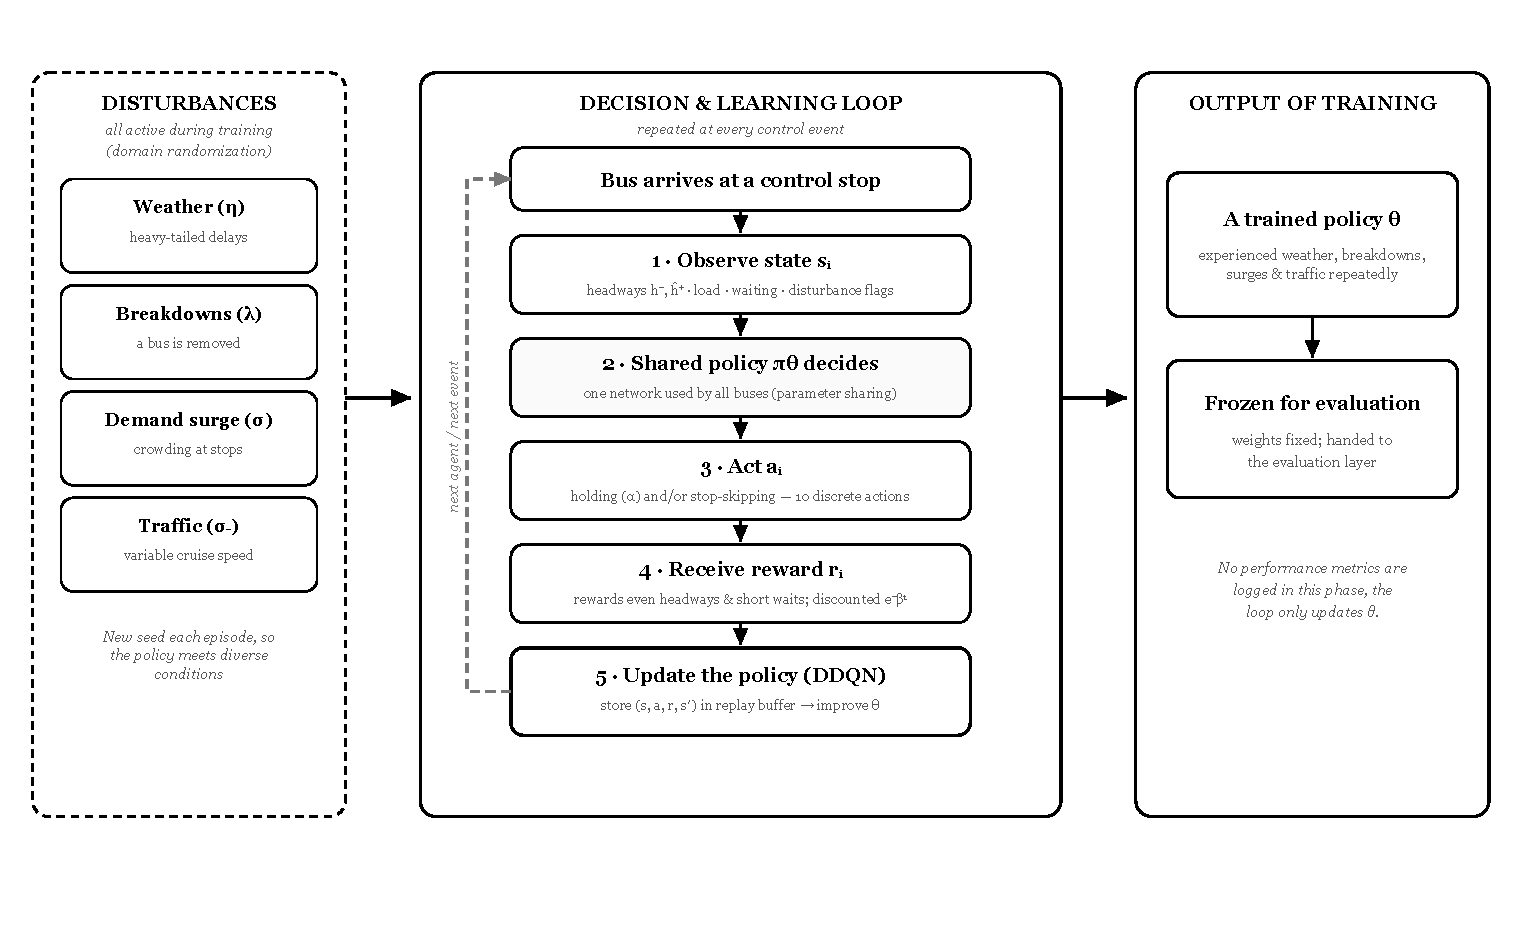
\includegraphics[width=\textwidth]{Figures/fig_3_2_aec_training.pdf}
    \caption[Agent--environment cycle (training)]{The asynchronous agent--environment
    cycle during training. Authors' illustration.}
    \label{fig:aec-training}
\end{figure}
 

Because heavy-tailed returns can destabilize value-based learning if injected without safeguards \cite{Henderson2018Matters,Agarwal2021Precipice}, training under disturbance is paired with the stabilizers discussed in Section~\ref{sec:challenges}: DDQN's double estimator, reward clipping, and slow target-network updates. If training under the full disturbance set proves unstable at the highest intensities despite these measures, a curriculum that ramps disturbance intensity over the course of training~\cite{Tang2024Curriculum} is retained as a fallback.

\clearpage

\subsection{Baseline Controllers for Comparison}

The MARL policy is benchmarked against three baseline controllers: \textbf{No Control (NC)}, \textbf{Forward Headway (FH)}, and \textbf{Even Headway (EH)}. These are the standard benchmark set in the MARL bus-control literature; both Wang and Sun \cite{Wangsun} and Rodriguez et al.~\cite{Rodriguez2023Cooperative} use this trio. Using the same baselines makes the results directly comparable to published work.

\subsubsection{No Control (NC)}

No holding or skipping is applied. Each bus dwells only for the time required to serve boarding and alighting passengers, then departs immediately. NC isolates uncontrolled behavior under each activation-matrix condition. If MARL cannot beat NC, the learned intervention is not operationally justified. Under combined disturbance, NC has no corrective mechanism for the added surge, weather, or breakdown stress.

\subsubsection{Forward Headway (FH)}

The classical holding rule introduced by Daganzo~\cite{Daganzo2009}. When a bus arrives at a control stop, its holding time is:

\begin{equation}
d_{FH} = \max\!\left\{0,\, \bar{d} + g\,(H_0 - h^-)\right\}
\label{eq:fh}
\end{equation}

where $H_0$ is the desired (scheduled) headway, $h^-$ is the forward headway (time gap to the bus ahead), $\bar{d}$ is the average slack delay at equilibrium, and $g > 0$ is a control gain parameter. If a bus is running closer to the bus ahead than scheduled ($h^- < H_0$), it holds for an additional period proportional to the gap deficit; if it is already at or beyond the desired spacing ($h^- \geq H_0$), it does not hold. Parameters $\bar{d}$ and $g$ follow Daganzo's original values. FH represents local, single-agent reactive control: each bus reacts only to information about the bus immediately ahead. Because Eq.~\eqref{eq:fh} conditions only on $h^-$, FH is expected to partially correct demand- and traffic-induced bunching but to respond poorly to a breakdown: it has no observation of the enlarged gap a failed bus leaves for the bus behind it, so the trailing bus's holding decision is uninformed by the breakdown until the irregularity has already propagated back to it.

\subsubsection{Even Headway (EH)}

A more globally aware rule that holds buses to equalize the forward and backward gaps simultaneously, following Rodriguez et al.~\cite{Rodriguez2023Cooperative}:

\begin{equation}
T_{EH} = \max\!\left\{\min\!\left[\frac{\hat{h}^+ - h^-}{2},\; 0.4\,H_0\right],\, 0\right\}
\label{eq:eh}
\end{equation}

where $h^-$ is the forward headway, $\hat{h}^+$ is the estimated backward headway (time gap to the bus behind), and $\frac{\hat{h}^+ - h^-}{2}$ is the holding time that would split the difference evenly between the two gaps. The hold is capped at $0.4\,H_0$ (40\% of the scheduled headway), the bound Rodriguez et al.\ used to prevent excessive intervention. This cap matches the maximum value in the MARL action set $\Omega = \{0, 0.1, 0.2, 0.3, 0.4\}$, so EH and MARL are constrained to the same maximum hold and the comparison is fair. EH represents globally-aware reactive control: it uses information about both neighbors but follows a fixed rule rather than a learned policy. Because Eq.~\eqref{eq:eh} is a fixed linear rule computed from the currently observed gaps, EH is expected to handle breakdowns better than FH, since the enlarged backward gap $\hat{h}^+$ enters the rule directly, but it has no mechanism to anticipate or discount the heavier-tailed delays that the weather generator introduces, since the rule was not designed with a heavy-tailed disturbance in mind.
\clearpage
\subsubsection{Baseline Comparisons}

The three controllers span the comparison space. NC tests whether intervention helps at all. FH tests whether MARL outperforms classical local reactive control. EH tests whether MARL outperforms classical global reactive control and EH is the stronger of the two classical baselines, consistently reported as the best non-RL controller in the literature \cite{Wangsun,Rodriguez2023Cooperative}. The acceptance criterion for the MARL policy in Stage A (Section~\ref{subsec:evaluation}) is therefore stated relative to EH: matching or beating EH is the meaningful test.

This three-way comparison also allows the study to attribute MARL's advantage. If MARL beats NC but not FH or EH, the benefit is from intervening, not from learning. If MARL beats FH but not EH, the benefit is from global awareness, not from learning. Only if MARL beats EH does the benefit come from the learned policy itself. The same logic applies in Stage B: the disturbance-handling claim is meaningful only if MARL's advantage over EH grows with $\eta$, since both controllers see the same disturbance realizations.

State-of-the-art MARL methods such as CAAC and IQNC-M \cite{Wangsun} were considered as additional baselines but excluded. Including them would shift the research question from ``does the declared MARL controller remain robust on Route 801?'' to ``which MARL variant is best?'', a different question requiring a larger algorithm-comparison budget.

\subsection{Data Analysis Methods}

The three response variables logged per run are defined as follows. \textbf{Mean passenger waiting time} ($\bar{W}$) is the average time elapsed from a passenger's arrival at a stop to their successful boarding, averaged across all passengers served and all stops over one simulated operating day:

\begin{equation}
\bar{W} = \frac{1}{P} \sum_{p=1}^{P} \left(t_p^{\text{board}} - t_p^{\text{arrive}}\right)
\label{eq:waiting_time}
\end{equation}

where $P$ is the total number of passengers served in the run and $t_p^{\text{board}}$, $t_p^{\text{arrive}}$ are the boarding and arrival times of passenger $p$. \textbf{Mean total travel time} ($\bar{T}$) is the average elapsed time from a bus's departure from the origin terminal to its arrival at the final stop of the sub-corridor, averaged across all bus trips completed during the simulated day. \textbf{Headway coefficient of variation} ($CV_h$) measures headway regularity:

\begin{equation}
CV_h = \frac{\sigma_h}{\mu_h}
\label{eq:headway_cv}
\end{equation}

where $\sigma_h$ and $\mu_h$ are the standard deviation and mean of observed inter-bus headways recorded at all stops over one simulated operating day. $CV_h = 0$ denotes perfectly regular headways; larger values indicate increasing bunching severity. This construction mirrors the baseline coefficient of variation $CV_0$ already defined for travel time (Table~\ref{tab:notation}), applied here to the headway distribution instead.

For each (control strategy, condition) cell, $N_{\mathrm{runs}} \geq 30$ independent Monte Carlo runs are executed using matched random seeds across strategies. Three response variables are logged per run: mean passenger waiting time, mean total travel time, and headway coefficient of variation. The minimum supplies repeated-run variance estimates but does not by itself guarantee normality under heavy tails; distribution checks and bootstrap confidence intervals are therefore required \cite{Wasserman2004,Agarwal2021Precipice}.

Statistical significance of performance differences between controllers will be assessed at a significance level of $\alpha = 0.05$. Because the same random seeds are reused across controllers within a disturbance level, comparisons between two controllers at the same disturbance level are naturally paired: the only difference between two runs is the controller, not the disturbance realization. Paired-sample tests will therefore be used for within-disturbance-level comparisons; unpaired tests will be used where seed matching does not apply (for example, comparing the same controller across different disturbance levels). Multiple-comparison correction will be applied across the four controllers to control the family-wise error rate.

For every disturbed condition, performance degradation is computed relative to the same controller's D+T Stage A result. Confidence intervals on the degradation ratio are computed by bootstrap resampling because ratios of means can be skewed under heavy-tailed stress \cite{EfronTibshirani1993}. Hypothesis tests, normality diagnostics, family-wise correction, bootstrap replicate count, and random seeds are fixed in the analysis configuration before final evaluation, following reinforcement-learning evaluation guidance \cite{Henderson2018Matters,Agarwal2021Precipice}. Run logs and analysis code are version-controlled; large generated outputs are checksum-recorded but not committed.

\subsection{Evaluation Methods}
\label{subsec:evaluation}



\textbf{Stage A: baseline evaluation.} The frozen MARL policy and three baselines are evaluated under D+T, with S/W/B off, for $N_{\mathrm{runs}}\geq30$ matched seeds. This is a stochastic empirical baseline rather than an ``ideal'' deterministic corridor. Parity with EH on waiting time and improvement over NC on headway variation remain the minimum acceptance targets.

\paragraph{Stage A acceptance criterion}
\begin{itemize}
\item[(i)] Mean passenger waiting time no worse than EH (no statistically significant degradation at $p < 0.05$ with multiple-comparison correction), and ideally a statistically significant improvement.
\item[(ii)] A statistically significant reduction in headway coefficient of variation relative to NC.
\end{itemize}

\begin{figure}[htbp]
    \centering
    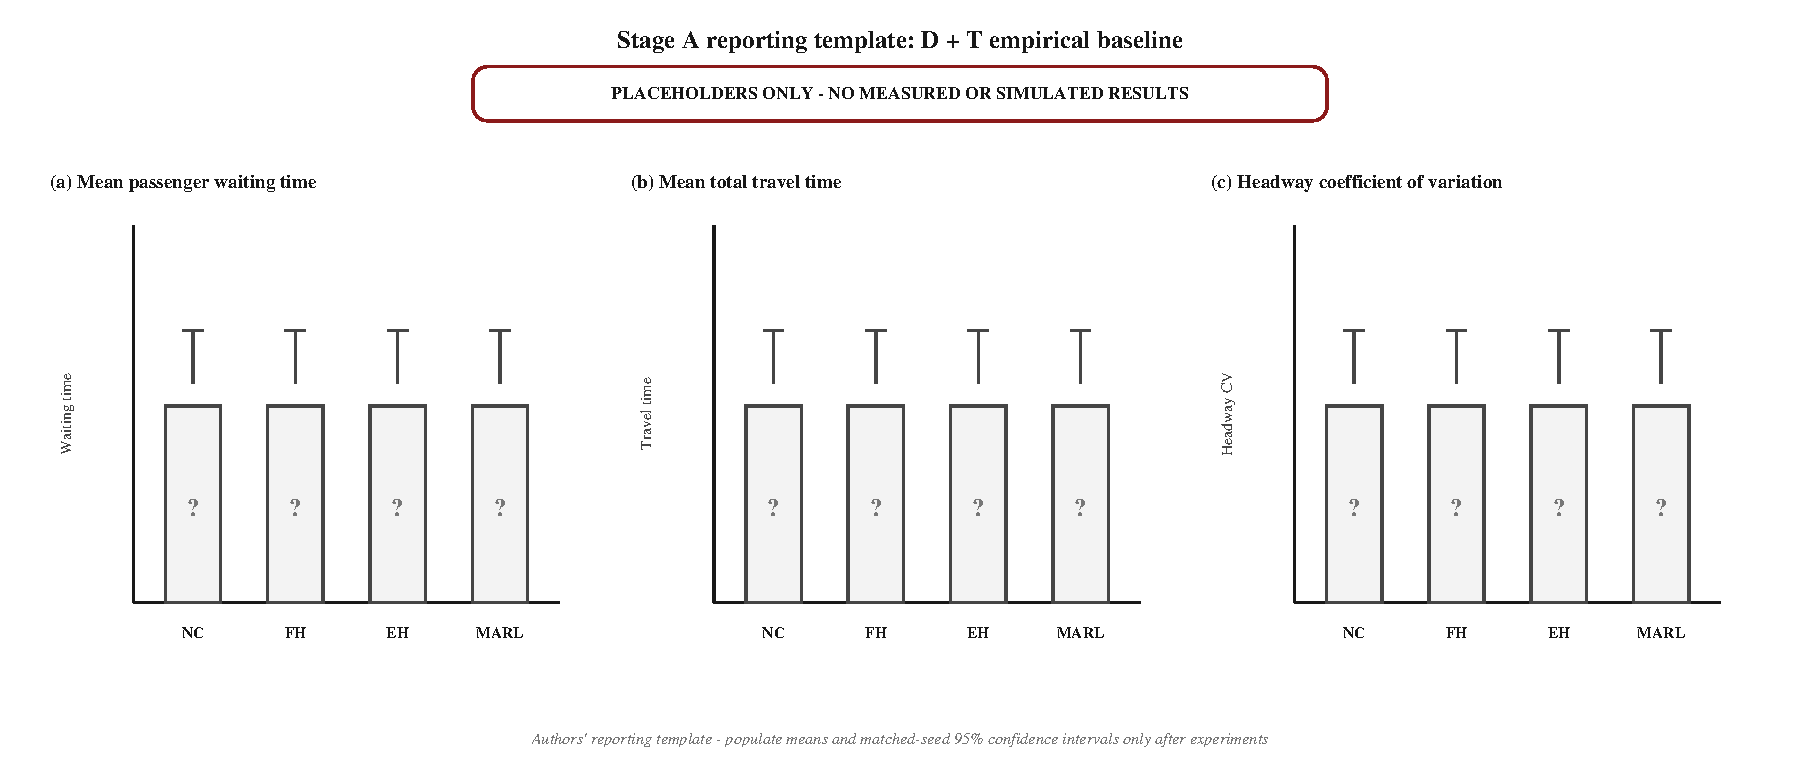
\includegraphics[width=0.8\textwidth]{Figures/meth_fig_eo3_1_ideal_results.pdf}
    \caption[Illustrative Stage A output format]{Illustrative output of the Stage A
    D+T baseline evaluation, comparing the four controllers (NC, FH, EH,
    MARL) across the three response variables: (a) mean passenger waiting time,
    (b) mean total travel time, and (c) headway coefficient of variation. Error
    bars represent 95\% confidence intervals over $N \geq 30$ Monte Carlo runs
    with matched seeds. Numerical values shown are illustrative and do not
    reflect measured results. Authors' illustration.}
    \label{fig:stage-a-illustrative}
\end{figure}

\textbf{Stage B: combined-disturbance evaluation.} Controllers are evaluated under D+T+S+W+B. One series uses the observed ordinary-rain exposure/multiplier; a separate extrapolative series sweeps synthetic $\eta\in\{0.3,0.6,1.0,1.3\}$. Each controller/condition cell has $N_{\mathrm{runs}}\geq30$ matched seeds. Outputs include response means and intervals, degradation relative to the same controller's Stage A result, and MARL's paired advantage over the strongest baseline. Single-disturbance ablations evaluate D+T+S, D+T+W (observed ordinary-rain definition), and D+T+B. Synthetic $\eta$ results are never relabeled as observed weather categories.

\paragraph{Stage B acceptance criterion} The MARL policy is reported as performing well under disturbance if its mean waiting time stays below that of the best-performing baseline across the full sweep, with statistical significance under the same correction as Stage A.

\begin{figure}[htbp]
    \centering
    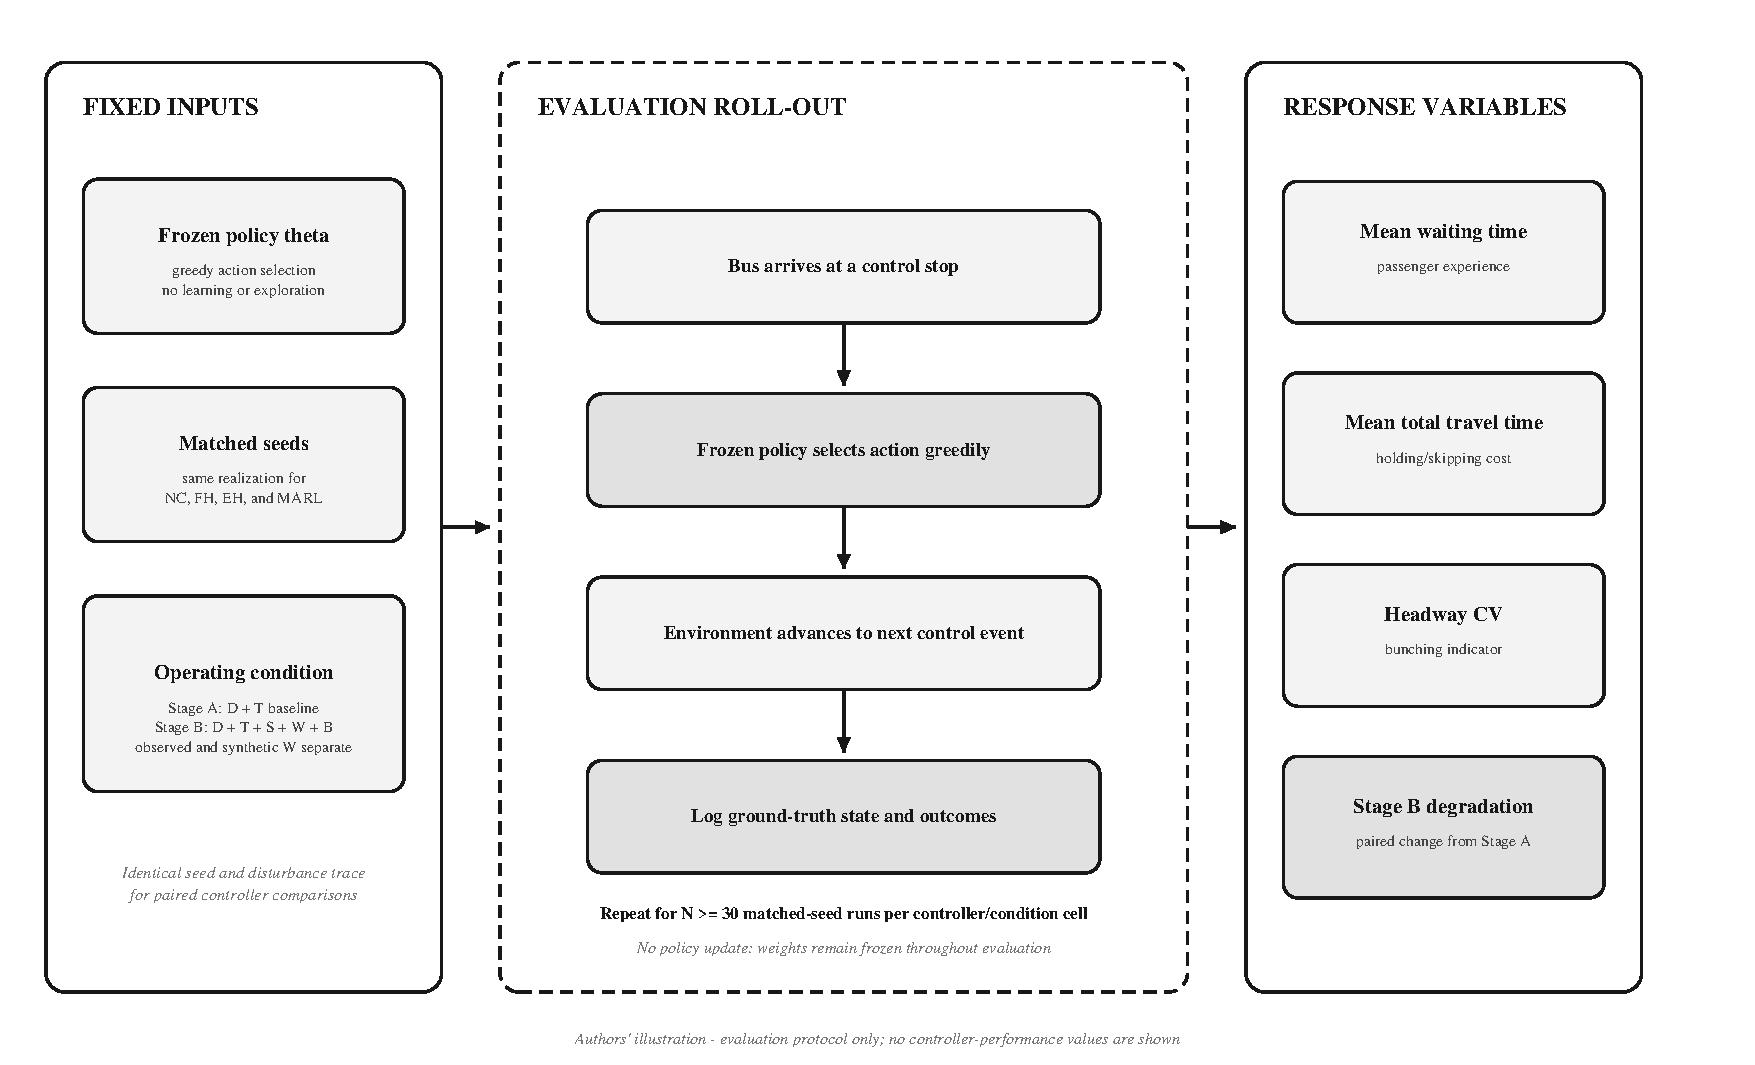
\includegraphics[width=1\textwidth]{Figures/fig_3_2b_aec_evaluation.pdf}
    \caption[Monte Carlo evaluation layer]{The Monte Carlo evaluation layer. The frozen policy $\theta$ selects the highest-valued action at each control stop without exploration or weight updates. Matched seeds ensure that every controller faces the same disturbance realization, so performance differences reflect the control strategy alone. Three response variables are recorded per run: mean passenger waiting time, mean total travel time, and headway coefficient of variation. Authors' illustration.}
    \label{fig:aec-eval}
\end{figure}


\section{Methodological Challenges}
\label{sec:challenges}

Three challenges shape the experimental design. The design is scoped to remain feasible on accessible hardware (a single cloud-notebook GPU runtime), and a tiered scope plan (stated at the end of this section) guarantees a defensible minimum deliverable even if the full sweep cannot be completed.

\textbf{Q-value overestimation under heavy-tailed returns.} Value-based methods such as DQN overestimate Q-values \cite{vanHasselt2016DDQN}, and this bias grows when returns are heavy-tailed, as they are under high-intensity disturbance \cite{Henderson2018Matters,Agarwal2021Precipice}. The DDQN double estimator addresses this by decoupling action selection from evaluation \cite{vanHasselt2016DDQN}. Because disturbances are active during training, reward clipping and target-network soft updates are used as additional stabilizers throughout, not only at the highest intensities.

\textbf{Computational cost.} At the minimum $N_{\mathrm{runs}}=30$, Stage A requires $4\times30=120$ runs. The observed-weather combined cell adds 120; the four-level synthetic combined sweep adds $4\times4\times30=480$; and the three single-disturbance ablations add $3\times4\times30=360$. The declared minimum is therefore 1{,}080 evaluation runs. SUMO is restricted to calibration, while event-driven evaluation is parallelized across seeds. Any reduced tier must preserve Stage A, the observed-weather combined cell, and at least one synthetic out-of-support level, and must be reported as a scope reduction rather than silently changing the matrix.

\textbf{Timeline feasibility.} The declared minimum evaluation suite contains 1{,}080 runs, as calculated above. No wall-clock duration is claimed before the Route 801 event-driven simulator is profiled: representative Stage A, observed-weather, synthetic-weather, and breakdown episodes will be benchmarked first, and the measured per-run CPU time, memory use, and training throughput will determine the parallelization and hardware plan. Rodriguez et al.~\cite{Rodriguez2023Cooperative} report a two-phase $500+300$-episode training design, but that external episode count is a sizing reference rather than evidence of this implementation's runtime. If the measured cost requires a reduced tier, it must preserve Stage A, the observed-weather combined cell, at least one synthetic out-of-support level, and the declared matched-seed comparison; every omitted cell must be reported as a scope reduction rather than silently changing the activation matrix.
